% Overview of the ai_learning repository.
% Build: latexmk -pdf repo_overview.tex   (from docs/slides/)
\documentclass[aspectratio=169,10pt]{beamer}
\usetheme[progressbar=frametitle, numbering=fraction]{metropolis}
\usepackage[T1]{fontenc}
\usepackage{lmodern}
\usepackage{booktabs}
\usepackage{listings}
\usepackage{tikz}
\usetikzlibrary{positioning, arrows.meta, fit}

\definecolor{accent}{HTML}{1F6F8B}
\definecolor{soft}{HTML}{E8F1F4}
\setbeamercolor{frametitle}{bg=accent}
\setbeamercolor{progress bar}{fg=accent!60}
\setbeamercolor{alerted text}{fg=accent}

\lstset{basicstyle=\ttfamily\scriptsize, keywordstyle=\color{accent}\bfseries,
        commentstyle=\color{gray}, stringstyle=\color{teal!70!black},
        language=R, columns=fullflexible, keepspaces=true, showstringspaces=false,
        frame=none, backgroundcolor=\color{soft}}

\newcommand{\code}[1]{\texttt{#1}}

\title{ai\_learning}
\subtitle{Current state of the repository}
\date{November 2026}

\begin{document}

\maketitle

% ---------------------------------------------------------------------------
\begin{frame}{What the repo does}
  \begin{columns}[T]
    \column{0.48\textwidth}
      \alert{1. Data setup} \\[2pt]
      Downloads review datasets locally, ready for cleaning.
      \begin{itemize}
        \item Amazon Reviews 2023 (34 categories)
        \item IMDB 50K movie reviews (Kaggle)
      \end{itemize}
    \column{0.48\textwidth}
      \alert{2. AI prompter} \\[2pt]
      Runs a fixed conversation with an LLM over every row of a dataset and saves the replies.
      \begin{itemize}
        \item Claude, ChatGPT, Gemini
        \item Offline mock model for dry runs
      \end{itemize}
  \end{columns}
  \vfill
  \begin{itemize}
    \item Written in \alert{R}; only needs \code{curl} and \code{jsonlite}
    \item Data and results stay \alert{out of git} (\code{0\_Data/} is ignored)
  \end{itemize}
\end{frame}

% ---------------------------------------------------------------------------
\begin{frame}[fragile]{Repository structure}
\begin{lstlisting}[language={}, columns=fixed, basicstyle=\ttfamily\footnotesize]
ai_learning/
|-- ai_learning.Rproj          RStudio project
|-- 0_Data/                    datasets + LLM results (git-ignored)
|-- 1_Data_Cleaning/
|   |-- setup_data.R           entry point: download datasets
|   `-- 1_Functions/           config, downloads, loaders
|-- 2_AIPrompter/
|   |-- run_prompter.R         entry point: run prompts over data
|   `-- 1_Functions/           providers, retries, prompter, output
`-- wiki/                      GitHub wiki pages
\end{lstlisting}
  \vspace{4pt}
  Each folder has \alert{one script you run}; helpers in \code{1\_Functions/} only define functions.
  Scripts find the repo themselves, whatever the working directory.
\end{frame}

% ---------------------------------------------------------------------------
\begin{frame}{1. Data setup: \code{setup\_data.R}}
  \begin{columns}[T]
    \column{0.55\textwidth}
      Interactive Amazon menu:
      \begin{enumerate}
        \item table of categories with \alert{download sizes}, marking files you \alert{already have}
        \item pick categories (\code{1,3,5-7}, names, \code{all}) and parts (reviews / metadata)
        \item confirm the total size
      \end{enumerate}
      Then the IMDB CSV. Re-runs skip existing files.
    \column{0.42\textwidth}
      \small
      \begin{tabular}{@{}ll@{}}
        \toprule
        Dataset & Stored as \\
        \midrule
        Amazon reviews & \code{.jsonl.gz} \\
        Amazon metadata & \code{.jsonl.gz} \\
        IMDB 50K & \code{.csv} \\
        \bottomrule
      \end{tabular}
      \vspace{8pt}

      Loaders: \code{load\_amazon\_reviews()}, \code{load\_amazon\_meta()}, \code{load\_imdb()}
  \end{columns}
\end{frame}

% ---------------------------------------------------------------------------
\begin{frame}{2. AI prompter: the conversation}
  \centering
  \resizebox{0.9\textwidth}{!}{%
  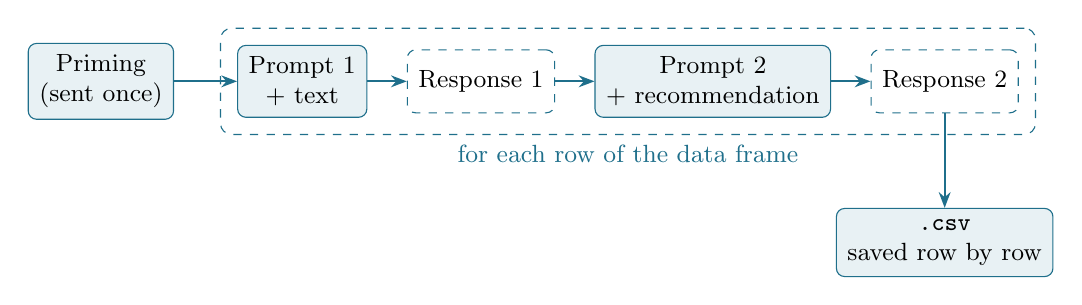
\begin{tikzpicture}[
      box/.style={draw=accent, fill=soft, rounded corners=3pt, minimum height=8mm,
                  align=center, font=\small, inner sep=4pt},
      reply/.style={box, fill=white, dashed},
      arr/.style={-{Stealth[length=2mm]}, accent, thick}]
    \node[box] (prime) {Priming\\(sent once)};
    \node[box, right=8mm of prime] (p1) {Prompt 1\\+ text};
    \node[reply, right=5mm of p1] (r1) {Response 1};
    \node[box, right=5mm of r1] (p2) {Prompt 2\\+ recommendation};
    \node[reply, right=5mm of p2] (r2) {Response 2};
    \draw[arr] (prime) -- (p1);
    \draw[arr] (p1) -- (r1);
    \draw[arr] (r1) -- (p2);
    \draw[arr] (p2) -- (r2);
    \node[draw=accent, dashed, rounded corners, fit=(p1)(r2), inner sep=6pt,
          label={[font=\small, text=accent]below:for each row of the data frame}] {};
    \node[box, below=12mm of r2] (csv) {\code{.csv}\\saved row by row};
    \draw[arr] (r2.south) -- (csv.north);
  \end{tikzpicture}}
  \vfill
  \begin{itemize}\small
    \item Any data frame: columns by name or number; one pair with \code{prompt\_one()}
    \item Per-row conversations (default) or one \code{continuous} conversation
    \item Export: \code{.csv}, \code{.txt} transcript, \code{.rds}, \code{.arrow} / \code{.parquet}
  \end{itemize}
\end{frame}

% ---------------------------------------------------------------------------
\begin{frame}[fragile]{2. AI prompter: usage}
\begin{lstlisting}
provider <- llm_provider("claude")       # "chatgpt", "gemini", "mock"
prompts  <- prompter_prompts(
  priming  = "You will read product reviews...",
  prompt_1 = "Summarise this review:",
  prompt_2 = "The recommendation was: {recommendation}. Does it match?")

results <- run_prompter(my_data, prompts, provider,
                        text_col = "review", recommendation_col = "recommend",
                        output_file = "0_Data/ai_prompter/my_run.csv")

one <- prompt_one("Great value.", "Would recommend", prompts, provider)
\end{lstlisting}
  \vspace{2pt}
  API keys live in \code{\char`\~/.Renviron} (\code{ANTHROPIC\_API\_KEY}, \code{OPENAI\_API\_KEY}, \code{GEMINI\_API\_KEY}), never in the repo.
\end{frame}

% ---------------------------------------------------------------------------
\begin{frame}{2. AI prompter: when things go wrong}
  \small
  \begin{tabular}{@{}p{0.36\textwidth}p{0.58\textwidth}@{}}
    \toprule
    Problem & What happens \\
    \midrule
    Reply cut off by token limit & Model asked to continue; parts joined \\
    Rate limit, overload, server error & Wait and retry (server's suggested delay or back-off) \\
    Out of credits / quota, bad key & Run stops cleanly; \alert{rerun the same call to resume} \\
    Conversation too long & Row marked as error, or oldest rows dropped (continuous) \\
    Service down & Stops after 3 failed rows in a row \\
    \bottomrule
  \end{tabular}
  \vfill
  Every row is written as soon as it finishes, so a crash or \code{Ctrl+C} loses nothing.
\end{frame}

% ---------------------------------------------------------------------------
\begin{frame}{Status and next steps}
  \begin{columns}[T]
    \column{0.48\textwidth}
      \alert{Done and tested}
      \begin{itemize}\small
        \item Data setup: merged into \code{main}
        \item Prompter: all failure cases tested on a local stand-in for each API
        \item Real Claude and Gemini APIs accept the request format
      \end{itemize}
    \column{0.48\textwidth}
      \alert{Open}
      \begin{itemize}\small
        \item Wiki pages and prompter not yet merged into \code{main}
        \item No real run with an API key yet
        \item Check default models in \code{config.R}
        \item Wiki pages for the prompter
        \item Optional: run rows in parallel
      \end{itemize}
  \end{columns}
\end{frame}

\end{document}
